\documentclass[a4paper,12pt]{article}
\usepackage[T1]{fontenc}
\usepackage[utf8]{inputenc}
\usepackage[english,russian]{babel}
\usepackage{pdfpages}
\usepackage{amsmath,amsfonts,amssymb,amsthm,mathtools}
\usepackage[left=10mm, top=10mm, right=10mm, bottom=20mm, nohead, nofoot]{geometry}
\usepackage{wasysym}
\author{\LARGEМерзляков Арсений}
\title{Анализ функции}
\pagestyle {empty}
\begin{document}
\maketitle
\begin{flushleft}
\Large
$f(x) = \ln {((\sin {(x)}+1.000))}$

Посчитаем то, что считается устно в садике - производную:

$g(x) = 1.000$

Ньютон перевернулся бы в гробу, если бы узнал, что ты не знаешь, что:

$g^{'}(x) = 0.000$

$g(x) = x$

Ллойд и Гарри из 'Тупой и ещё тупее' знали, что:

$g^{'}(x) = 1.000$

$g(x) = \sin {(x)}$

Если бы моя собака умела говорить, то сказала бы, что:

$g^{'}(x) = \cos {(x)} \cdot 1.000$

$g(x) = (\sin {(x)}+1.000)$

Если бы меня разбудили в ночь после посвята, то я бы сходу ответил, что:

$g^{'}(x) = (\cos {(x)} \cdot 1.000+0.000)$

$g(x) = \ln {((\sin {(x)}+1.000))}$

В садике мне рассказывали, что:

$g^{'}(x) =  \dfrac{1.000}{(\sin {(x)}+1.000)}  \cdot (\cos {(x)} \cdot 1.000+0.000)$

После очевиднейших упрощений, которые адекватный человек может сделать ещё в утробе, получаем:

$ \dfrac{1.000}{(\sin {(x)}+1.000)}  \cdot \cos {(x)}$

Выполним самую тривиальную вещь в курсе математического анализа - разложение функции по формуле Тейлора: 

$f(x) = ((((x+ \dfrac{(-1.000) \cdot (x)^{2.000}}{2.000} )+ \dfrac{(x)^{3.000}}{6.000} )+ \dfrac{(-2.000) \cdot (x)^{4.000}}{24.000} )+ \dfrac{5.000 \cdot (x)^{5.000}}{120.000} ) + o(x^{5}), x \rightarrow 0$

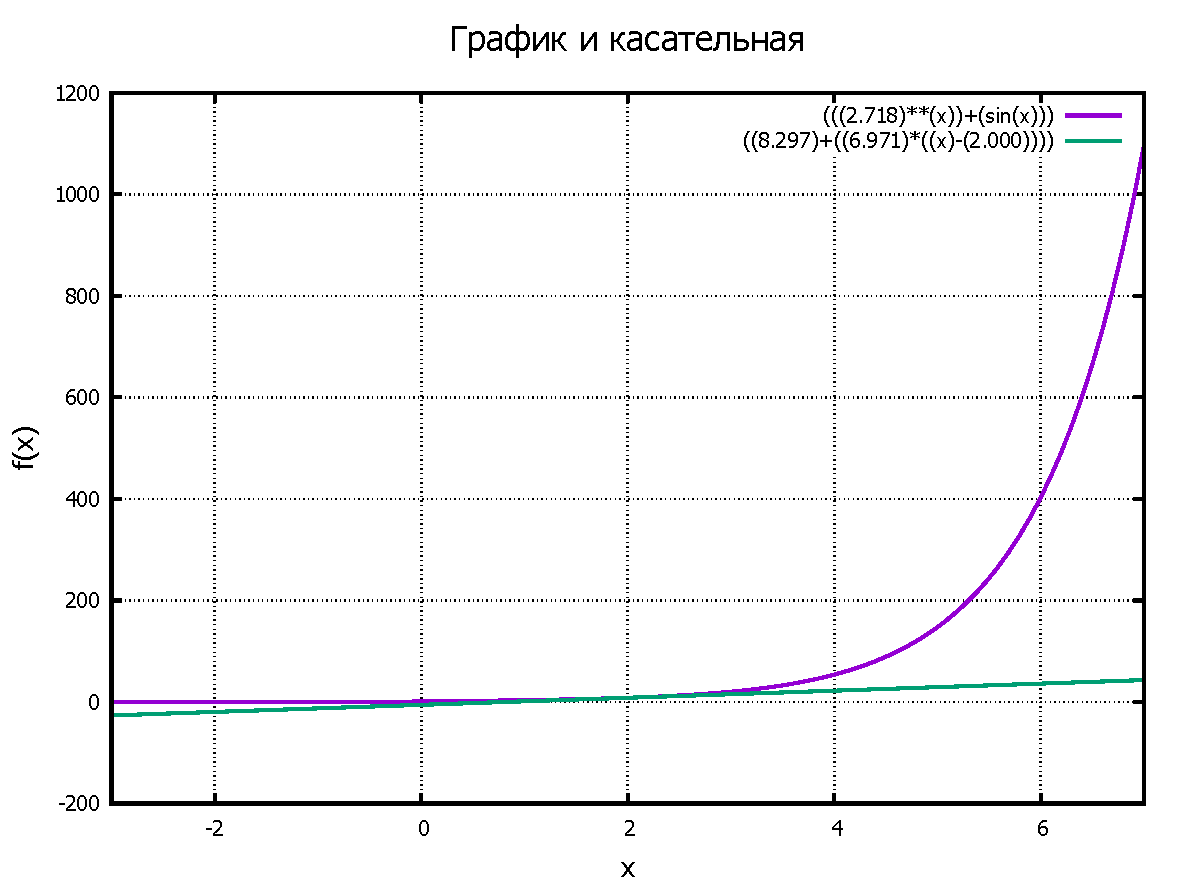
\includepdf[pages=-]{latex/graph1.pdf}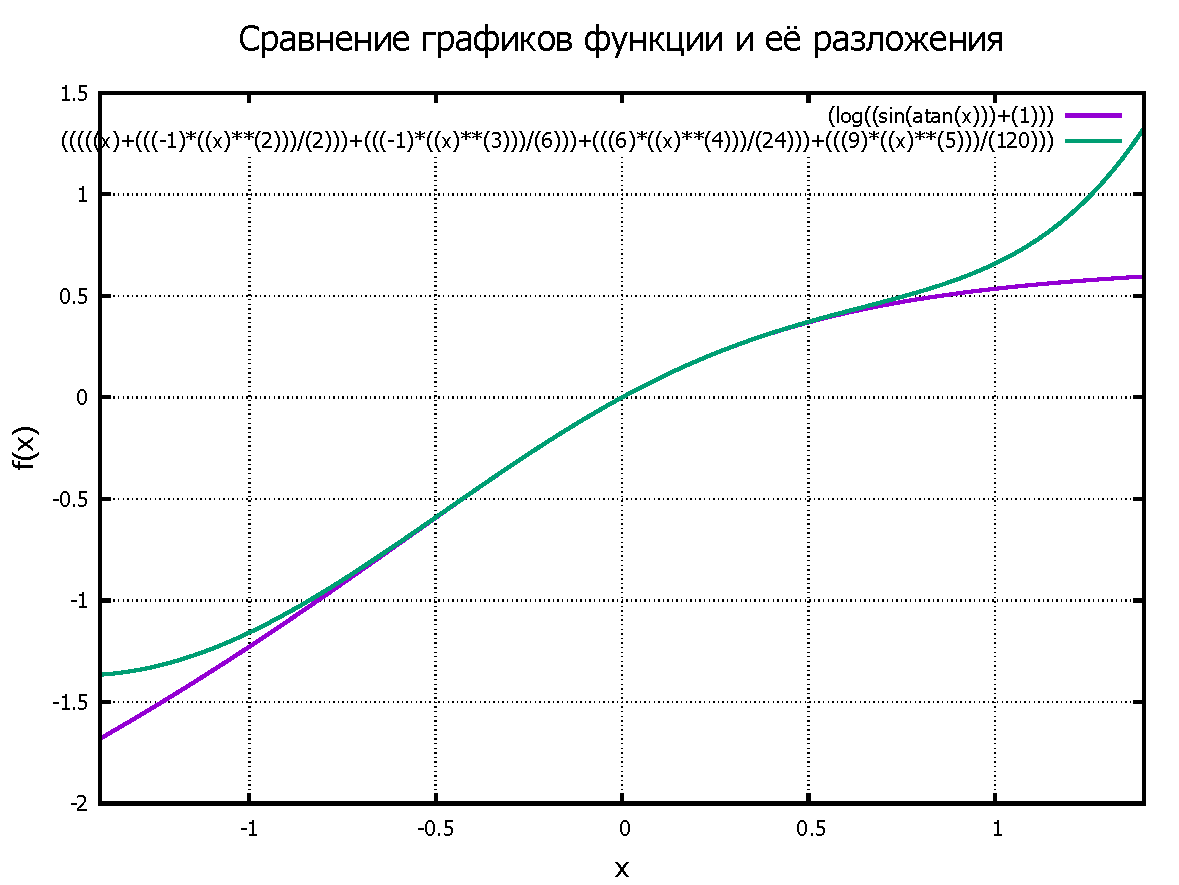
\includepdf[pages=-]{latex/graph2.pdf}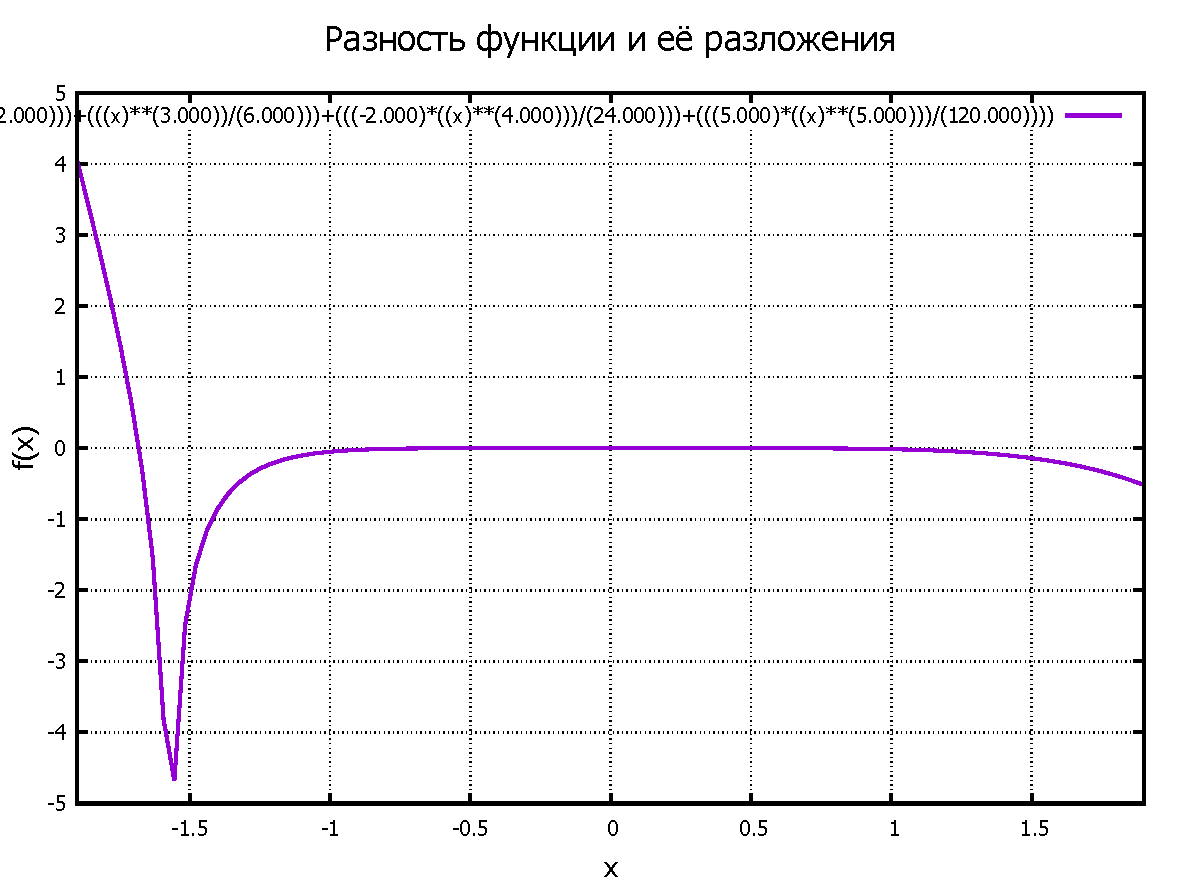
\includepdf[pages=-]{latex/graph3.pdf}\end{flushleft}
\end{document}